\documentclass{article}

% for choosing the proper font encoding
\usepackage[T1]{fontenc}
% for proper encoding
\usepackage[utf8]{inputenc}
% enhanced font Latin Modern
\usepackage{lmodern}
% multi-language support
\usepackage[english]{babel}
% for inline and display quotations.
\usepackage[autostyle]{csquotes}
\usepackage{csquotes}
% set the default 4 inches margin to be 1 inch
\usepackage{fullpage}
% for colorful link
\usepackage[ocgcolorlinks,pdfusetitle]{hyperref}
% for doi link
\usepackage{doi}
%
\usepackage{filecontents}

\usepackage{amsmath, amssymb, amsthm, graphicx, epsfig, fancyhdr, enumitem}
\usepackage{setspace}
\newtheoremstyle{break}
  {\topsep}{\topsep}%
  {\itshape}{}%
  {\bfseries}{}%
  {\newline}{}%
\theoremstyle{break}
\newtheorem{theorem}{Theorem}[section]
\newtheorem{lemma}{Lemma}[section]
\doublespacing

% for back reference in bibliography
\usepackage[backend=biber,style=authoryear]{biblatex}
\addbibresource{Random_Number_Generation.bib}


\begin{document}
\title{Linear Congruence Generators}
\author{Matthew Moreno}
\date{December 2, 2015}
\maketitle

\section{Introduction}
\subsection{Motivation}
In addition to the lottery \footnote{if it is being conducted fairly, at least!}, sequences of random numbers are necessary ingredients for Monte Carlo methods, digital cryptography, and computer simulations of phenomena with random aspects, and other applications. Over the years, several schemes to use physical phenomena that emulate the function of a mathematical random variable have been put forward. Notably, these include use of a ``sonic roulette wheel'' by the Rand Corporation to generate data for its book of ``a million random digits''\autocite{rand_corporation_million_2001}, the extraction of random digits from images of lava lamps in motion \autocite{noll_method_1998}, the use of human input (e.g. on the keyboard or mouse) to generate random digits  \autocite{cole_network_2011}, and the parsing of random streams of data from quantum effects such as the fluctuations in the magnetic field of a vacuum
 \autocite{_anu_????}. While these operations give good results in practice, they are expensive to implement and provide a slow and highly constrained bandwith of values. Thus, deterministic mathematical operations to generate sequences of numbers that emulate the distribution of numbers from an ideal random variable have been developed. These methods are commonly referred to as ``pseudorandom number generation.'' In general, these algorithms are launched with a ``seed'' value from which an initial internal state is generated. Then, a sequence is generated by repeatedly performing a deterministic computational operation on the state to transition to a new internal state and yield a new ``random'' value.
 It is important to note several important distinctions beetween pseudorandom number generation and true random generation. First, future values produced by a pseudorandom generator, unlike the future value of a true random variable, can be deduced from information on the current state of the pseudorandom generator---pseudorandom generation is a completely deterministic process. Also, unlike ideal random variables, sequences of numbers generated by pseudorandom methods are periodic. There are a finite number of internal states that a pseudorandom generator can be in so periodicity arises in the output of the generator when it eventually returns to a previously encountered internal state. John Von Neumann, who worked with early computing devices such as the ENIAC, commented on these important distinctions, noting that that ``any one who considers arithmetical methods of producing random digits is, of course, in a state of sin'' \autocite{neumann_various_1950}.
 The unique properties that differentiate pseudorandom generation from true random generation---determinism and periodicity---can be overcome or even employed gainfully in applied settings, however. The periodicity of sequences generated via pseudorandom generation can easily be made so large\footnote{The Mersenne twister, for example, exhibits a $2^{19937}-1$ element long periodic in its output.} that it is of no practical concern \autocite{matsumoto_mersenne_1998}. The determinism of pseudorandom generation allows, so long as the initial seed value is known, for a pseudorandom sequence to be recreated so the computations performed using that particular sequence can be readily repeated. This is particularly useful in the debugging process \autocite{hull_random_1962}. Further, the use of pesuedorandom generation frees computer scientists from expensive, specialized hardware required to perform true random number generation and the physically-limited throughput capacity of true random number generation. It should be no surprise, therefore, that pseudorandom generation is widely employed today in applications ranging from financial simulation to biological simulation to digital playlist shuffling \autocite{schwartz_biological_2008, dunbar_stochastic_????}.

\subsection{The Linear Congruence Method} The Linear Congruence Method (LCM) is a well-studied approach to pseudorandom number generation. It was developed by Lehmer in 1949. Using a multiplier of 23 and a modulus of $10^{8} + 1$, he successfully generated sequences of more than five million eight decimal digit numbers using an ENIAC computing machine \autocite{hull_random_1962}. This method has a solid theoretical framework showing that, under certain special circumstances, the sequence possesses the very similar moments to the uniform distribution over (0,1]. Additionally, by strategically choosing the modulus as a power of two, the calculations required to perform the linear congruence method can be performed rather efficiently with binary computing machines. $m$-tuples derived from sequences generated using Linear Congruence method have been shown to lie on relatively few hyperplanes in $\mathbb{R}^m$ \autocite{marsaglia_random_1968}. Thus, because the values of a member of a LCM-generated sequence are not completely statistically independent of the other values in the sequence, the LCM approach is not appropriate for applications highly sensitive to the quality of pseudorandom sequences that are provided (such as Monte Carlo methods). Although this approach has been largely superseded by a new generation of pseudorandom generators such as the Mersenne Twister, it is still not infrequently employed today, and is of theoretical interest and historical significance.

\section{The Linear Congruence Method}
\subsection{Algorithm}
The Linear Congruence Method algorithm is presented as shown in \autocite{hull_random_1962}. Begin by choosing ``magic values'' as follows:
\begin{itemize}
\item \textbf{m}: modulo; $m > 0, m \in \mathbb{Z}$ 
\item \textbf{a}: multiplier; $a > 0, a \in \mathbb{Z}$
\item \textbf{c}: increment; $c \geq 0, a \in \mathbb{Z}$
\end{itemize}
The particular choice of ``magic values'' determines important characteristics of the sequence $\{\mathbb{X}_i\}$ that will be generated using LCG. This will be discussed in greater detail later, but suffice it to say that a poor choice of ``magic values'' may lead to relatively short periodicity in $\{\mathbb{X}_i\}$ while choosing ``magic values'' that fulfill certain criteria guarantees a periodicity of exactly $m$, the modulo value chosen.

Next, a seed value $\mathbb{X}_0$ is chosen such that $\mathbb{X}_0 < m$ and $\mathbb{X}_0 \in \mathbb{Z}$. The sequence $\{\mathbb{X}_i\}$ is then generated recursively using the relationship
\begin{equation} \label{eq:lgp_rec_rel}
\mathbb{X}_{n+1} = (a \cdot \mathbb{X}_{n} + c) \mod m
\end{equation}
In this way, the sequence $\{\mathbb{X}_i\}$ can be built up term after term as desired; this relationship is typically employed in applications using the LCM method. However, a closed-form expression can also be used to determine the $n$th value of a sequence $\{\mathbb{X}_i\}$ with seed $\mathbb{X}_0$
\begin{equation} 
\mathbb{X}_{n} = \Big( a^n \mathbb{X}_0 + \frac{(a^n - 1)c}{a-1} \Big) \mod m 
\end{equation}
This type of ``shortcut'' is useful in applications where  distinct, finite subsequences of a single pseudorandom sequence with a certain seed are utilized asynchronously, such as GPU computing\autocite{_mwc64x_????}, as well as in formal mathematical analysis of the properties of the Linear Congruence Method.
\subsection{Computational Examples}
Table~\ref{short_period_comp_examp} provides a first example of a sequence generated by the Linear Congruence Method with $m = 5$, $a=3$, $c=2$, $\mathbb{X}_0 = 1$.
\begin{table}[htbp]
\centering
\begin{tabular}{l|c|c}
$n$ & $\mathbb{X}_n$ & $(\mathbb{X}_n \cdot a + c) \mod m$  \\\hline
0 & 1 &  $(1 \cdot 3 + 2) \mod 5 = 0$ \\
1 & 0 &  $(0 \cdot 3 + 2) \mod 5 = 2$ \\
2 & 2 &  $(2 \cdot 3 + 2) \mod 5 = 3$ \\
3 & 3 &  $(3 \cdot 3 + 2) \mod 5 = 1$ \\
4 & 1 &   \\
\end{tabular}
\caption{An annotated sequence of numbers generated using the linear congruence method with period $p < m$.}
\label{short_period_comp_examp}
\end{table}
Note that after only four steps in this sequence, we have returned to a value already encountered in the sequence. Because---by definition---the value of each item $\mathbb{X}_n$ where $n > 0$ in the sequence $\{\mathbb{X}_i\}$ depends only on the value of the item in the sequence that directly precedes it, $\mathbb{X}_{n-1}$, the sequence will exhibit a periodicity with period $p = 4$. Observe further that $p < m$ and, relatedly, that there does not exist $n$ such that $\mathbb{X}_n = 4$. 

Table~\ref{long_period_comp_examp} provides a second, and final, example of a sequence generated by the Linear Congruence Method with $m = 9$, $a = 4$, $c = 2$ $\mathbb{X}_0 = 2$.
\begin{table}[htbp]
\centering
\begin{tabular}{l|c|c}
$n$ & $\mathbb{X}_n$ & $(\mathbb{X}_n \cdot a + c) \mod m$  \\\hline
0 & 4 &  $(4 \cdot 4 + 2) \mod 9 = 0$ \\
1 & 0 & $(0 \cdot 4 + 2) \mod 9 = 2$ \\
2 & 2 & $(2 \cdot 4 + 2) \mod 9 = 1$ \\
3 & 1 & $(1 \cdot 4 + 2) \mod 9 = 6$ \\
4 & 6 & $(6 \cdot 4 + 2) \mod 9 = 8$ \\
5 & 8 & $(8 \cdot 4 + 2) \mod 9 = 7$ \\
6 & 7 & $(7 \cdot 4 + 2) \mod 9 = 3$ \\
7 & 3 & $(3 \cdot 4 + 2) \mod 9 = 5$ \\
8 & 5 & $(5 \cdot 4 + 2) \mod 9 = 4$ \\
9 & 4 & \\
\end{tabular}
\caption{An annotated sequence of numbers generated using the linear congruence method with period $p = m$.}
\label{long_period_comp_examp}
\end{table}
After nine steps in this sequence, we have to returned to a value already encountered in the sequence. Thus, this sequence will exhibit periodicity with period $p = 9$. Take special note that, for this particular set of ``magic values'' we have $p = m$ and with $0 \leq j,k < m$ for every $k$ there exists a unique $j$ such that $\mathbb{X}_k = j$ and vice versa.\footnote{Equivalently, a one-to-one bijective relation exists between $\{\mathbb{X}_i\}$ where $0 \leq i < p$ and $\{n\}$ where $0 \leq i < n$.} As discussed in Section \ref{sec:distribution}, these observations hold true for any possible choice of seed value $\mathbb{X}_0$ and result from fulfillment of particular conditions on the ``magic values'' chosen for the Linear Congruence Generator.
\section{Distribution of Random Variables Simulated Using the Linear Congruence Method} \label{sec:distribution}
We begin by introducing a theorem from \autocite{hull_random_1962} in order to facilitate our investigation into the distribution of sequences $\{\mathbb{X}_i\}$ generated via LCM.
\begin{theorem}[Linear Congruence Generator Full Period Theorem] \label{thm:full_period}
The sequence generated by the recursive relationship shown in Equation \ref{eq:lgp_rec_rel} has period length $p = m$ if and only if
\begin{enumerate}
\item $c$ is relatively prime to $m$;
\item for all prime factors $f$ of $m$, $a \mod f = 1$;
\item if 4 is a factor of $m$, $a \mod 4 = 1$.
\end{enumerate}
\end{theorem}
This theorem will allow us to reckon out the $k$th raw moment of a scaled form of a sequence $\{\mathbb{X}_{i}\}$ produced from a Linear Congruence Generator with ``magic numbers'' that fulfill the conditions of Theorem \ref{thm:full_period} and thus have period length $p = m$. With $\{\mathbb{X}_{i}\}$ defined as a sequence generated from a Linear Congruence Generator with modulo $m$ and ``magic numbers'' satisfying the stipulations of Theorem \ref{thm:full_period}, define the sequence $\{\mathbb{Y}_{i}\}$ such that
\begin{equation} \label{eqn:scaled_lcs}
 \mathbb{Y}_{n} = \frac{\mathbb{X}_{n}}{m} ~ \forall n
\end{equation}
A value $\mathbb{X}_n$ in a sequence $\{\mathbb{X}_i\}$ from a Linear Congruence Generator with modulo $m$ is inherently restricted $0 \leq \mathbb{X}_n < m$ so $\mathbb{Y}_{n} \in [0,1) ~ \forall n$. Theorem \ref{thm:lcm_kth_mom} gives us $\lim_{m \rightarrow \infty} E(\{\mathbb{Y}_{i}\}^k) = 1/(k+1)$ if we assume special conditions on the ``magic numbers'' governing the LCM generator behind $\{\mathbb{Y}_{i}\}$. First, though, we develop Lemmas \ref{lma:uniq_val} and \ref{lma:comp_lcm_full_per_seq}.
\begin{lemma}[Uniqueness of Values of Sequences Generated Via LCM] \label{lma:uniq_val}
Let $p$ represent the smallest periodicity of a sequence $\{\mathbb{X}_i\}$ from a Linear Congruence Generator. All values $\mathbb{X}_0\}, ..., \mathbb{X}_{p-1}$ are unique.
\end{lemma}
\begin{proof}
Suppose there exists $0 \leq j,k < p$ such that $i \neq j$ and $\mathbb{X}_j = \mathbb{X}_k$. For convenience, we assume without loss of generality that $j < k$ By the recursive definition $\ref{eq:lgp_rec_rel}$ of the sequence $\{\mathbb{X}_i\}$, for elements $s$ and $t$ of the sequence $\mathbb{X}_{s} = \mathbb{X}_{t}$ implies $\mathbb{X}_{s+1} = \mathbb{X}_{t+1}$. Thus, by induction with base case $\mathbb{X}_j = \mathbb{X}_k$, for all $n > 0 \in \mathbb{Z}$ we have $\mathbb{X}_{j+n} = \mathbb{X}_{k+n}$. Rewriting, we have $\mathbb{X}_{j+n} = \mathbb{X}_{j+(k-j)+n}$ for all $n > 0 \in \mathbb{Z}$. It follows by further inductive analysis that $\mathbb{X}_{j+n} = \mathbb{X}_{j+\alpha(k-j)+n}$ for any $\alpha > 0 \in \mathbb{Z}$. Take note that with $j,k < p$ we have $k - j < p$. The existence of $0 \leq j,k < p$ such that $\mathbb{X}_j = \mathbb{X}_k$ therefore implies the existence of periodicity $k - j < p$ in the sequence $\mathbb{X}_i$. Our initial supposition therefore violates the status of $p$ as the smallest periodicity of a sequence $\{\mathbb{X}_i\}$, so it cannot be true.
\end{proof}

\begin{lemma}[Composition of Full Period Sequences Generated Via LCM] \label{lma:comp_lcm_full_per_seq}
Let $p$ represent the smallest periodicity of a sequence $\{\mathbb{X}_i\}$ from a Linear Congruence Generator with modulo $m$. If the sequence $\{\mathbb{X}_i\}$ achieves maximal period-length, that is if $p = m$, the subsequence $\{\mathbb{X}_i\}$ with $i \in \mathbb{Z}$ and $0 \leq i < p$ is a re-arrangement of the sequence $0, ..., p - 1$.
\end{lemma}
\begin{proof} 
We want to show that for every $0 \leq n < p$ with $n \in \mathbb{Z}$ there exists a unique $i \in \mathbb{Z}$ with $0 \leq i <p$ such that $\mathbb{X}_i = n$. Lemma 3.1 gives us uniqueness; there cannot exist $0 \leq j,k < p$ such that $i \neq j$ and $\mathbb{X}_j = \mathbb{X}_k$. Existence, however, remains untreated. We will first show $q \in \{\mathbb{X}_i\} \Rightarrow q \in \{0, ..., p - 1\}$ then verify existence by showing $q \in \{0, ..., p - 1\} \Rightarrow q \in \{\mathbb{X}_i\}$.

\begin{itemize}

\item $q \in \{\mathbb{X}_i\} \Rightarrow q \in \{0, ..., p - 1\}$ \\
Recall that, by the definition of the modulo operation, a value $\mathbb{X}_n$ in a sequence $\{\mathbb{X}_i\}$ from a Linear Congruence Generator with modulo $m$ is restricted $0 \leq \mathbb{X}_n < m$. As an assumption, we have $p = m$ so the restriction on $\mathbb{X}_n$ can be written as $0 \leq \mathbb{X}_n < p$. With $\mathbb{X}_n \in \mathbb{Z}$ we have $q \in \{0, ..., p - 1\}$.

\item $q \in \{0, ..., p - 1\} \Rightarrow q \in \{\mathbb{X}_i\}$ \\
Suppose there exists $q \in \{0, ..., p - 1\}$ such that $q \notin \{\mathbb{X}_i\}$. We have $g \in \{\mathbb{X}_i\} \Rightarrow g \in \{0, ..., p - 1\}$ so we would have $g \in \{\mathbb{X}_i\} \Rightarrow g \in \{\{0,...,p-1\} \setminus \{q\}\}$. Thus, we would have $\{\mathbb{X}_i\} \subset {\{0, ..., p - 1\} \setminus \{q\}}$. Note that $\left\vert{\{\mathbb{X}_i\}}\right\vert = \left\vert{\{0, ..., p - 1\}}\right\vert = p$. Because $q \in \{0, ..., p - 1\}$, $\left\vert{\{0, ..., p - 1\} \setminus \{q\}}\right\vert = p - 1$. Uniqueness of $\mathbb{X}_n \in \{\mathbb{X}_i\}$ together with $g \in \{\mathbb{X}_i\} \Rightarrow g \in \{\{0,...,p-1\} \setminus \{q\}\}$ would force $\left\vert{\{\mathbb{X}_i\}}\right\vert \leq p - 1$. However, we know $\left\vert{\{\mathbb{X}_i\}}\right\vert = p$. Thus, it must be true that $q \in \{0, ..., p - 1\} \Rightarrow q \in \{\mathbb{X}_i\}$.
\end{itemize}

\end{proof} 

\begin{theorem}[Linear Congruence Method Sequence kth Raw Moment] \label{thm:lcm_kth_mom}
With $\{\mathbb{Y}_{i}\}$ defined via Equation \ref{eqn:scaled_lcs} with a Linear Congruence Generator with ``magic numbers'' satisfying Theorem \ref{thm:full_period}, $\lim_{m\rightarrow\infty}E(\{\mathbb{Y}_{i}\}^k) = 1/(k+1)$.\footnote{Indirectly inspired by \autocite{schruben_ieor_2007}.}
\end{theorem}
\begin{proof}

From a frequentist perspective it makes sense to calculate the $k$th moment of a  random variable simulated by a sequence $\{\mathbb{S}_i\}$ as $\lim_{a\rightarrow \infty} \sum_{n = 0}^{a}\frac{\mathbb{S}_{n}^k}{n}.$ If the sequence $\{\mathbb{S}_i\}$ has periodicity $p$, we calculate the expected value of a random variable simulated a sequence $\{\mathbb{S}_i\}$ as 
\[
E(\{\mathbb{S}_i\}) = \frac{1}{p} \sum_{n = 0}^{p-1} \mathbb{S}_n^k
\]
Note that we can choose an arbitrarily large $m$ and find values of $c$ and $a$ that fulfill Theorem \ref{thm:full_period}. Consider, for example, defining $m = 3^z$ with $z > 1, z \subset \mathbb{Z}$, $c$ as 2, and $a$ as 2. We have $\lim_{z \rightarrow \infty} m = \lim_{z \rightarrow \infty} 3^z = \infty$ so $m$ is unbounded.
With the unbounded nature of $m$ in hand define $\{\mathbb{X}_{i}\}$ as the sequence generated by a linear congruence generator with ``magic values'' satisfying Theorem \ref{thm:full_period} such that $\{\mathbb{X}_{i}\}$ takes on its full periodicity $m$. Define sequence $\{\mathbb{Y}_i\}$ such that each term $\mathbb{Y}_n = \mathbb{X}_n/m$.
\[
\lim_{m \rightarrow \infty} E(\{\mathbb{Y}_i\}^k) = \lim_{m \rightarrow \infty} \frac{1}{m} \sum_{n = 0}^{m-1} \mathbb{Y}_n^k = \lim_{m \rightarrow \infty} \frac{1}{m} \sum_{n = 0}^{m-1} (\mathbb{X}_n/m)^k = \frac{1}{m^{k+1}} \sum_{n = 0}^{m-1} \mathbb{X}_n^k
\]
Lemma \ref{lma:comp_lcm_full_per_seq} gives us that the subsequence $\{\mathbb{X}_i\}$ with $i \in \mathbb{Z}$ and $0 \leq i < p$ is a re-ordering of the sequence $0, ..., p - 1$ so we rearrange to find
\[
\lim_{m \rightarrow \infty} E(\{\mathbb{Y}_i\}^k) = \lim_{m \rightarrow \infty} \frac{1}{m^{k+1}} \sum_{n = 0}^{m-1} n^k
\]
At this point, we bring in Faulhaber's formula to do some heavy lifting
\[
\sum_{n=1}^{N} n^{k} = \frac{1}{k+1} \sum_{j=0}^{k} (-1)^j {k+1 \choose j} B_j N^{k+1-j}
\]
where $B_j$ is the $j$th Bernoulli number. Rewriting our expression for the $k$th raw moment of $\{\mathbb{Y}_i\}$ with Faulhaber's formula yields
\[
\lim_{m \rightarrow \infty} E(\{\mathbb{Y}_i\}^k) = \lim_{m \rightarrow \infty} \frac{1}{m^{k+1}} \frac{1}{k+1} \sum_{j=0}^{k} (-1)^j {k+1 \choose j} B_j (m-1)^{k+1-j} + \frac{1}{m^{k+1}}
\]
Removing elements that disappear as $m \rightarrow \infty$, our expression cleans up to
\[
\lim_{m \rightarrow \infty} E(\{\mathbb{Y}_i\}^k) = \lim_{m \rightarrow \infty} \frac{1}{m^{k+1}} \frac{1}{k+1} (-1)^0 {k+1 \choose 0} B_0 (m-1)^{k+1} 
\]
Further evaluation and simplification, including use of the identity $B_0 = 1$, yields
\[
\lim_{m \rightarrow \infty} E(\{\mathbb{Y}_i\}^k) = \frac{1}{k+1}
\]
\end{proof}
Remark that our results from Theorem \ref{thm:lcm_kth_mom} give, with $\{\mathbb{Y}_i\}$ defined via Equation \ref{eqn:scaled_lcs}
\[
\lim_{m\rightarrow\infty}E(\{\mathbb{Y}_{i}\}) = 1/2
\]
and 
\[
\lim_{m\rightarrow\infty}var(\{\mathbb{Y}_{i}\}) = E(\{\mathbb{Y}_{i}\}^2) - (E(\{\mathbb{Y}_{i}\}))^2 = 1/3 - (1/2)^2 = 1/12 
\]
These values match exactly the expected value and the variance of the uniform random distribution $U[0,1)$.Next, we will obtain an expression for the $k$th raw moment of the uniform random distribution $U[0,1)$ in order to perform a more rigorous comparison between a random variable simulated via a sequence $\{\mathbb{Y}_{i}\}$ and $U[0,1)$.
\begin{theorem}[Uniform Random Distribution Kth Moment] \label{thm:urd_kth_mom}
For $\mathbb{U} \sim U[0,1)$, $E(\mathbb{U}^k) = 1/(1+k)$.
\end{theorem}
\begin{proof}
Take $\mathbb{U} \sim U[0,1)$ and let $f(x)$ represent the probability distribution of $\mathbb{U}$. By definition,
\[
E(\mathbb{U}^k) = \int_{-\infty}^{\infty} f(x) \cdot x^k dx
\]
For a uniform random distribution over $[0,1)$, we have $f(x) = 1$ for $x$ on $[0,1)$ and $f(x) = 0$ otherwise. Thus,
\[
E(\mathbb{U}^k) = \int_{0}^{1} x^k dx = \left. \frac{x^{k+1}}{k+1} \right|_0^1 = \frac{1}{k+1}
\]
\end{proof}
Theorems \ref{thm:lcm_kth_mom} and \ref{thm:urd_kth_mom} reveal that the $k$th moments of a random variable distributed as $U[0,1)$ and a random variable simulated via $\{\mathbb{Y}\}_i$ (as defined in Equation \ref{eqn:scaled_lcs}) for large $m$ are both given as $1/(1+k)$. Moment generating functions can be used as a unique identifying feature of a probability distribution \autocite{dunbar_stochastic_????}. The identical results of Theorems  \ref{thm:lcm_kth_mom} and \ref{thm:urd_kth_mom} thus draw strong similarities between the behavior of distributions of a random variable $~ U[0,1)$ and a random variable simulated via $\{\mathbb{Y}\}_i$. Our analysis leads us to conclude that, for large $m$ and selection of ``magic numbers'' that satisfy Theorem \ref{thm:full_period} the distribution of a random variable simulated using the Linear Generation Method very well resembles the unit uniform distribution $U[0,1)$.

\section{Independence and Random Variables Simulated Using the Linear Congruence Method}
Linear Congruence Generators suffer from inherent correlations between consecutive elements of the sequences they generate, as shown by  \autocite{marsaglia_random_1968}. Thus, sequences generated through the Linear Congruence Method do not truly display independence and should not be used for sensitive applications such as Monte Carlo methods. However, with the right choice of ``magic values,'' Linear Congruence generators can still perform ``well enough'' to pass many, except the most rigorous, statistical tests for randomness. We will begin this section by briefly discussing Theorem \ref{thm:main_in_plane}, a well known result from  \autocite{marsaglia_random_1968}, before moving along to touch on results from statistical tests for randomness.
\begin{theorem}[Random Numbers Fall Mainly In the Planes] \label{thm:main_in_plane}
If $c_1,c_2,...,c_n$ is any choice of integers such that
\[ 
c_1 + c_2k + c_3k^2 + ... + c_n k^{n-1} \equiv 0 \mod m
\]
then all of the points $\pi_1,\pi_2,...$ will lie i the set of parallel hyperplanes defined by the equations
\[
c_1x_1 + c_2x_2 + ... + c_nx_n = 0, \pm 1, \pm 2, ...
\]
There are at most
\[
|c_1| + |c_2| + ... + |c_n|
\]
of these hyperplanes which intersect the unit n-cube, and there is always a choice of $c_1,c_2,...,c_n$ such that all of the points fall in fewer than $(n!m)^{1/n}$ hyperplanes.
\end{theorem}
Theorem \ref{thm:main_in_plane} essentially tells us that plots of $n$-tuples of consecutive values in a LCM derived in a $n$-dimensional space are arranged in a highly ordered fashion. Specifically, they are restricted to a bounded number of distinct hyperplanes. The result of this theorem can readily be appreciated visually.
\begin{figure}[!tbp]
  \centering
  \begin{minipage}[b]{0.4\textwidth}
  \centering
    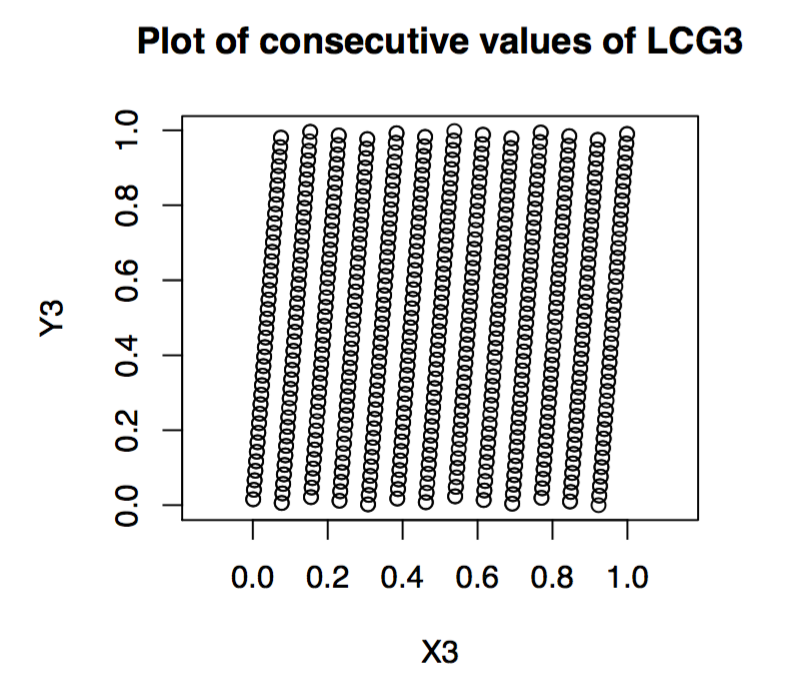
\includegraphics[width=\textwidth]{LCG3_consecutive_values.png}
    \label{fig:high_correlation}\caption{A plot of consecutive values showing egregious correlations in a sequence generated via the Linear Congruence Method \autocite{burgoine_testing_2013}.}  \end{minipage}
  \hspace{1 cm}
  \begin{minipage}[b]{0.4\textwidth}
 	 \centering
    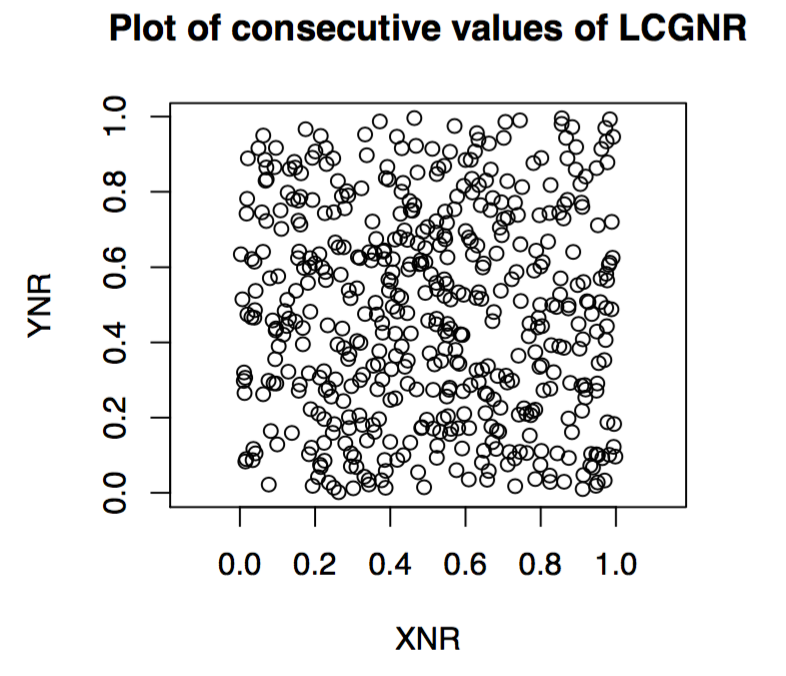
\includegraphics[width=\textwidth]{LCGNR_consecutive_values.png} \label{fig:low_correlation}\caption{ A plot of consecutive values from a sequence generated using the Linear Congruence Method  with little visually apparent correlations \autocite{burgoine_testing_2013}.}
  \end{minipage}
\end{figure}
Consider Figure 1; it is apparent that significant correlation exists between consecutive values (in the form of diagonal ``streaks'') in a sequence generated by the LCG3 generator (a LCM generator with specific ``magic values''). In Figure 2, on the other hand, statistical tests confirm that, as we would expect from a cursory visual inspection, the correlations are not as egregious. Recall that Theorem $\ref{thm:main_in_plane}$ gives us the upper bound on the number of planes containing all $n$-tuples generated by as $(n!m)^{1/n}$. This bound decreases as $m$, the modulo component of the Linear Congruence Generator, decreases. As we would expect from visual comparison of Figures 1 and 2, $m$ for the LCG3 generator associated with Figure 1 is much smaller than the $m$ for the LCGNR generator associated with Figure 2 \autocite{burgoine_testing_2013}.

The question of how to evaluate the statistical performance of a pseudorandom generator is nebulous. The practical consensus, though, seems to be subjecting it to a battery of tests where each tests a specific statistical property of a random variable that would be expected to manifest in the series of values generated by a pseudorandom generator \autocite{lecuyer_testu01:_2007}. Testing a somewhat slaphazard series of null hypotheses, does not definitively affirm the quality of pseudorandom number generator. Instead this approach of trial by statistical battery simply looks for evidence that a sequence of numbers fails to fulfill a specific statistical property we desire. Examples of statistical tests that might be considered include comparison of the empirical distribution of the maximum streak lengths to the theoretical distribution of maximum streak lengths by a chi-square test or comparison of actual outcomes of a series of random walks (i.e. number of steps to the right, maximum distance reached, fraction of time spent to the right of the origin, number of returns to zero, and number of sign changes) to the expected theoretical distributions, also using a chi-square test \autocite{lecuyer_testu01:_2007}. In \autocite{burgoine_testing_2013}, Linear Congruence Generators with differing ``magic values'' were subjected to a battery of statistical probes such as Kolmogorov-Smirnov tests and the Spearman’s Rank Correlation Coefficient test. The performance of these generators fell on a wide spectrum, one passing all the tests and others failing differing numbers of tests. Although LCG statistical performance can be enhanced by an appropriate choice of ``magic numbers,'' it is still vastly outperformed by new, more sophisticated generators such as the Mersenne Twister \autocite{burgoine_testing_2013}. Thus, more sophisticated generators should be preferred in settings where the very high statistical quality of pseudorandom sequences is essential.  
\section{References}

% bibliography
\printbibliography[heading=none]
\end{document}

\begin{comment}
\begin{theorem}[Linear Congruence Method Sequence Expected Value] \label{thm:lcm_ex_val}
With $\{\mathbb{Y}_{i}\}$ defined via Equation \ref{eqn:scaled_lcs} with a Linear Congruence Generator with ``magic numbers'' satisfying Theorem \ref{thm:full_period}, $\lim_{m\rightarrow\infty}E(\{\mathbb{Y}_{i}\}) = 1/2$. 
\end{theorem}
\begin{proof}

From a frequentist perspective it makes sense to calculate the expected value of a  random variable simulated by a sequence $\{\mathbb{S}_i\}$ as $lim_{a\rightarrow \infty} \sum_{n = 0}^{a}\frac{\mathbb{S}_{n}}{n}.$ If the sequence $\{\mathbb{S}_i\}$ has periodicity $p$, we calculate the expected value of a random variable simulated a sequence $\{\mathbb{S}_i\}$ as 
\[
E(\{\mathbb{S}_i\}) = \frac{1}{p} \sum_{n = 0}^{p-1} \mathbb{S}_n
\]
Note that we can choose an arbitrarily large $m$ and find values of $c$ and $a$ that fulfill Theorem \ref{thm:full_period}. Consider, for example, defining $m = 3^z$ with $z > 1, z \subset \mathbb{Z}$, $c$ as 2, and $a$ as 2. We have $\lim_{z \rightarrow \infty} m = \lim_{z \rightarrow \infty} 3^z = \infty$ so $m$ is unbounded.
With the unbounded nature of $m$ in hand define $\{\mathbb{X}_{i}\}$ as the sequence generated by a linear congruence generator with ``magic values'' satisfying Theorem \ref{thm:full_period} such that $\{\mathbb{X}_{i}\}$ takes on its full periodicity $m$. Define sequence $\{\mathbb{Y}_i\}$ such that each term $\mathbb{Y}_n = \mathbb{X}_n/m$.
\[
\lim_{m \rightarrow \infty} E(\{\mathbb{Y}_i\}) = \lim_{m \rightarrow \infty} \frac{1}{m} \sum_{n = 0}^{m-1} \mathbb{Y}_n = \lim_{m \rightarrow \infty} \frac{1}{m^2} \sum_{n = 0}^{m-1} \mathbb{X}_n
\]
Lemma \ref{lma:comp_lcm_full_per_seq} gives us that the subsequence $\{\mathbb{X}_i\}$ with $i \in \mathbb{Z}$ and $0 \leq i < p$ is a re-arrangement of the sequence $0, ..., p - 1$ so we rearrange our expression as
\[
\lim_{m \rightarrow \infty} E(\{\mathbb{Y}_i\}) = \lim_{m \rightarrow \infty} \frac{1}{m^2} \sum_{n = 0}^{m-1} n
\]
Rewriting with the identity $\sum_{x=1}^N x^1 = 1/2 \cdot N (N+1)$ and simplifying yields
\[
\lim_{m \rightarrow \infty} E(\{\mathbb{Y}_i\}) = \lim_{m \rightarrow \infty} \frac{1/2 \cdot m (m+1)}{m^2} = 1/2
\]
\end{proof}


...


\subsection{Cellular Automata Method}
\autocite{wolfram_random_1986}
\subsubsection{Definition}
\subsubsection{Computational Example}
This example will probably include an image, because cellular automata is so photogenic.
\subsubsection{Discussion}
\subsection{Mersenne Twister}
\subsubsection{Definition}
As before.
\subsubsection{Computational Example}
As before.
\subsubsection{Discussion}
This section will discuss the theoretical framework of this method, touching on why (if it all) it is guaranteed to be uniformly distributed. This section will discuss its  properties with respect to k-distribution and might (?) include some Borel (?) stuff.
\autocite{makototakuji_m_matsumotonishimura_mersenne_????}
\subsection{Blum Blum Shum Method}
(If time allows... this might get cut out).\autocite{blum_simple_1986}
\subsubsection{Definition}
\subsubsection{Computational Example}
\subsubsection{Discussion}
\section{From Uniform Random Distribution to Other Distributions}
\subsection{Transformation Method} Schwartz 118 \autocite{schwartz_biological_2008} , also known as inverse transform sampling
This section will present the transformation method of relating a uniform distribution to an arbitrary probability distribution and provide a specific example of this relationship (perhaps with the exponential distribution).

\subsection{The Rejection Method} Schwartz 121
This section will present the rejection method of relating a uniform distribution to an arbitrary probability distribution and provide a specific example of this relationship (perhaps with the normal distribution).
case study: simulating normals using rejection Jones 347
\autocite{jones_introduction_2009}
\section{Statistical Tests for Randomness}
Empirical evaluation of the performance of pseudorandom number generators is essential verify the performance of novel approaches to RNG as well as to check for bugs in implementations of well-established RNG approaches. The RANDU debacle, in which a flawed pseudorandom number generator was widely deployed and used, evidences the importance of such testing. The question of how to evaluate the performance of a pseudorandom generator, though, is nebulous. The practical consensus, though, seems to be subjecting it to a battery of tests where each tests a specific statistical property of a random variable that would be expected to manifest in the series of values generated by a pseudorandom generator. We will be testing a somewhat slaphazard series of null hypotheses, so we will not be able to definitively affirm the quality of pseudorandom number generator. Instead we will be looking for evidence that a sequence of numbers fails to fulfill a specific property we desire. There is no limit on the amount of data we can collect besides the computing resources we are working with, so if we get a suspicious $p$ value we can continue testing until our suspicious dissipate or are more conclusively proven. 

In this section I will present a few (perhaps one or two?) specific statistical tests in depth. Candidates for this treatment include:
\begin{displayquote}
Longest run of 1’s. The longest head run test [Foldes 1979; Gordon et al. 1986] is a variant of the run test that looks at the length Y of the longest substring of successive 1’s in a string of length m. This is repeated n times and the empirical distribution of the n realizations of Y is compared with its theoretical distribution by a chi-square test. \autocite{lecuyer_testu01:_2007}
\end{displayquote}

Random Walk tests, which compare the actual outcomes of a series of random walks (i.e. number of steps to the right, maximum distance reached, fraction of time spent to the right of the origin, number of returns to zero, and number of sign changes) to the expected theoretical distributions using a chi-square test (there seem accessible to a thorough treatment using what we did in class)

\autocite{lecuyer_testu01:_2007}
\end{comment}
